% This version of CVPR template is provided by Ming-Ming Cheng.
% Please leave an issue if you found a bug:
% https://github.com/MCG-NKU/CVPR_Template.

%\documentclass[review]{cvpr}
\documentclass[final]{cvpr}
\usepackage{times}
\usepackage{epsfig}
\usepackage{graphicx}
\usepackage{amsmath}
\usepackage{amssymb}
\usepackage{svg}
\usepackage{subfig}
\usepackage[printonlyused, smaller]{acronym}
\usepackage{multirow}
\usepackage{makecell}
% Include other packages here, before hyperref.
\usepackage{algorithm}
\usepackage{algpseudocode}

% If you comment hyperref and then uncomment it, you should delete
% egpaper.aux before re-running latex.  (Or just hit 'q' on the first latex
% run, let it finish, and you should be clear).
\usepackage[pagebackref=true,breaklinks=true,colorlinks,bookmarks=false]{hyperref}


\def\cvprPaperID{****} % *** Enter the CVPR Paper ID here
\def\confYear{CVPR 2022}
%\setcounter{page}{4321} % For final version only


\begin{document}

%%%%%%%%% TITLE
\title{Camera Pose Estimation using Regression Forest and RANSAC Optimization}

\author{Falk Ebert\\
\tt 4018276\\
{\tt\small Physics M.Sc.}
% For a paper whose authors are all at the same institution,
% omit the following lines up until the closing ``}''.
% Additional authors and addresses can be added with ``\and'',
% just like the second author.
% To save space, use either the email address or home page, not both
\and
Jason Pyanowski\\
\tt 3663907\\
{\tt\small Data and Computer Science M.Sc.}
\and
Nadine Theisen\\
\tt 3475402\\
{\tt\small Physics M.Sc.}
\and
Marven Hinze\\
\tt 3664283\\
{\tt\small Data and Computer Science M.Sc.}
}

\maketitle


%%%%%%%%% ABSTRACT
\begin{abstract}
This project aims to realize the approach of~\cite{shotton2013} to infer the position and rotation of a camera
in the 3D world space given a set of 2D images. A regression forest is used to predict the correspondences between 
pixels and world coordinates using RGB and depth information. An initial set of hypothesized camera
poses are deduced by applying the regression forest and are then optimized with a preemptive RANSAC. The algorithm 
is evaluated on the 7-scenes dataset~\cite{glocker2013} which contains RGB images with corresponding depth
information for each pixel of 7 different 3D scenes. Subsequently, the ability of the forest to predict 2D-3D 
correspondences is evaluated. To verify the estimated camera poses of the RANSAC algorithm, the translational and 
angular error with respect to the known ground truths are measured. These findings are then compared to the results
of~\cite{shotton2013}. 
\end{abstract}

%%%%%%%%% BODY TEXT
\section{Introduction}
Inferring the pose of a camera in a known 3D environment is a crucial part of many up-to-date applications.
Especially in the area of robotics, where \ac{SLAM} algorithms are applied or in augmented reality a sufficiently precise 
estimate is required~\cite{shotton2013}. More recently, approaches using neural networks became present and provide
a fast estimation of the position and orientation of a camera~\cite{Blanton2020}. 

In this project, we provide an approach of interfering the pose of a camera in the world coordinate system
based on the work of Shotton et al.~\cite{shotton2013}. Therefore, a regression forest is utilized to find correspondences
between pixels in an image and world coordinates. Given a data set
consisting of RGB-D images as well as depth information for each pixel, the 3D world coordinate can be estimated.

Based on the predicted world coordinates the camera location and orientation is obtained by applying RANSAC
optimization. Initially, camera pose hypotheses are generated and subsequently refined using an energy function.
The hypothesis with the lowest energy term is considered as the final camera pose. 

The present approach does not require any deep understanding of the scene but completely relies on 
pixel-based features~\cite{shotton2013}. Additionally, only a small set of pixels is needed in order to estimate 
the camera pose, because the regression forest is trained on a sufficiently large data set. This allows to 
run the pose estimation on mobile devices or microcontrollers.

To evaluate the predictions of a forest, the 7-scenes dataset~\cite{glocker2013} set which consists of seven 
different scenes with each between $2,000$ and $12,000$ frames is utilized. To each frame the corresponding 
depth map and the ground truth camera pose is given which encodes position and orientation. The findings are 
compared to the results of~\cite{shotton2013} using the translational and angular error of 
the predicted to the ground truth camera poses for each scene in the data set.


%-------------------------------------------------------------------------
\subsection{Related Work}
Nowadays, many approaches to infer camera poses or poses of objects in general are based on either image-based approaches or 
sparse keypoint matching. The application of imaged-based pose estimation uses the whole image and matches different frames 
using high level features like \ac{SIFT} or \ac{SURF}~\cite{Klein2008}. Thereby, an initial camera pose is refined using 
the obtained features and known camera poses. The result is then calculated as a weighted average over the 
images that describe the camera pose best. 

More recently, approaches concerning sparse feature matching gained interest~\cite{Holzer2012}. Again, high level features are detected but 
instead matched with a large set of feature descriptors. This approach requires a lot of engineering regarding the feature
description and matching process. The routine of inferring a camera pose presented in the reference paper of Shotton et al.~\cite{shotton2013}
comes the difference that only low-level features are utilized. Simple pixel-based features are applied in order to train a
regression forest without the need of feature descriptors. The predictions of the camera pose are then made directly one the
output of the forest which correlates 3D image pixels with 3D world coordinates. The underlying forest can additionally be 
evaluated for abrbitrary pixel positions and is therefore sparse.


\section{Methods}
%-------------------------------------------------------------------------
This section gives an overview of the methods used in this project. We will discuss
the concept of regression forests including feature extraction and the RANSAC algorithm
used for estimating the camera pose from the image data. We will not discuss all aspects
in full detail but only provide further explanations where we find it relevant
for the presentation of our work and results.

\subsection{Data Preparation}
%-------------------------------------------------------------------------
To train the regression forest the 7-scenes dataset~\cite{glocker2013} is utilized. 
Each scene consists of multiple image sequences that cover the area of interest. Using RGB-D 
Kinect camera, depth information for each pixel is extracted. The resolution of the $24$ 
bit RGB-images is $640\times480$ pixels and the corresponding $16$ bit depth map is given 
in millimeters. For each image a $4\times4$ ground truth camera pose in homogenous coordinates 
is provided, which allows to validate the estimated camera pose matrix for a given image. 
Each dataset is split randomly into train and test. 

Based on that, our data set is composed of a number of samples $\{(\boldsymbol{p}_i, \boldsymbol{w}_i)\}$ with
$\boldsymbol{p}_i = (x_l, y_l)_i$ and $\boldsymbol{w}_i = (x_s, y_s, z_s)_i$ where the subscripts
$l$ and $s$ denote image pixel coordinates and scene coordinates respectively.\\

\subsection{Regression Forest}
%-------------------------------------------------------------------------

In this project we use a regression forest to predict scene coordinates for a given
sample image coordinate as suggested in \cite{shotton2013}. In this section we will
give some background on the concept of regression forests, the pixel coordinate
labeling and the image-feature extraction on which the forests base their predictions.\\

\subsubsection{Decision Trees}
%-------------------------------------------------------------------------
A regression forest consists of a number $N$ of regression trees, which each consist 
of root node and it's children~\cite{Criminisi2013}. We consider the special case of binary decision trees
where each node (unless it is a leaf node) has a left and a right child. Each node $n$
stores a set of parameters $\theta_n$ which are used in the calculation of a
feature response function $f_{\theta}(\boldsymbol{p}) \in \{1, 0\}$ which determines if the input
data point $\boldsymbol{p}$ is branched to the left or right child node. To every leaf node
(i.e. a node without children) we assign a response value $\boldsymbol{w}_n$ representing
the tree's prediction for a data point $\boldsymbol{p}$ that has reached this node. In our
specific application the input data points $\boldsymbol{p}$ are 2D pixel coordinates and the
responses $\boldsymbol{w}$ are 3D world coordinates.

The process of training the tree involves finding the set of parameters
$\{\theta_n | \, \forall \, \text{nodes} \, n\}$ which results in the best predictions
for previously unseen input data points $\boldsymbol{p}$. However, this final goal cannot
be optimized directly during training, as this would entail optimization in the
very large space of all possible parameters for all tree-nodes simultaneously. Therefor
it is much more efficient to optimize the parameters one node at a time using a
proxy-objective $Q(S_{\text{tot}},\, S_{\text{left}}(\theta),\, S_{\text{right}}(\theta))$
which ideally leads to a similar result.

Let $S_{\text{tot},n} = \{ (\boldsymbol{p}_i, \boldsymbol{w}_i) \, | \, i \in |S_n|\}$ denote the
input data and target response for a given node $n$. According to its parameters the
node splits this set into the subsets
\begin{equation}
\begin{split}
	S_{\text{left},n}(\theta_n) = \{(\boldsymbol{p}_i, \boldsymbol{w}_i) \,|\, f_{\theta_n}(\boldsymbol{p}_i) = 0\} \\
	S_{\text{right},n}(\theta_n) = \{(\boldsymbol{p}_i, \boldsymbol{w}_i) \,|\, f_{\theta_n}(\boldsymbol{p}_i) = 1\}
\end{split}
\end{equation}
corresponding to left and right child node respectively. The objective function $Q$ is
then used to assign a score to the split resulting from the parameters $\theta_n$ at
this node.

The objective function used here optimizes for a reduction in variance of the target 
responses (i.e. "wants the tree to group together points with similar scene coordinates").
Defining $W_n = \{ \boldsymbol{w}_i \, | \, (\boldsymbol{p}_i, \boldsymbol{w}_i) \in S_n \}$ this
objective can be mathematically expressed as:
\begin{multline}
	Q(W_\text{tot}, \theta) =
		\text{Var}(W_\text{tot})\, - \sum_{d\,\in\{\text{left,\,right}\}}
			\dfrac{|W_d(\theta)|}{|W_\text{tot}|} \text{Var}(W_d(\theta))\\
	\text{with} \hspace{5mm} \text{Var}(W) = |W|^{-1} \sum_{\boldsymbol{w}\in W} ||\boldsymbol{w} - \bar{\boldsymbol{w}}||_2^2
\end{multline}
Training the complete tree then involves choosing a set of images from which a number
of sample pixels is drawn. These samples are then evaluated (i.e. split into left and right set)
by the tree's root node for a number of parameter-sets. For each set of parameters, the
split's score is calculated using the objective function and the optimal parameters for
this node are recorded. The process is then repeated for the node's children with the corresponding
set (left or right; split according to the optimal parameters) until either the set contains
only one element or the maximum depth is reached.
When the maximum depth is reached and the set still contains more than one element, a response
needs to be calculated for the node. This response represents the tree's prediction for 
all pixels, which reach this node and is calculated from the sample's ground truth scene coordinates.
In practice, a mean shift variance algorithm \cite{Comaniciu2002} is used to find the center of the 
largest cluster. Thereby, at most $500$ random coordinates are utilized for calculation to limit 
the computational cost.

\subsubsection{Image Features}
%-------------------------------------------------------------------------
In order to use a decision tree to infer scene coordinates from the pixel coordinates,
it is necessary to calculate features associated with a given pixel coordinate from the
image data. This is implemented in the feature response function mentioned earlier.
We have chosen to use the 'Depth-Adaptive RGB' image features from \cite{shotton2013} which
is defined as
\begin{equation}
	f_{\theta}^{da-rgb}(\boldsymbol{p}) = I\left(\boldsymbol{p} + \frac{\boldsymbol{\delta}_1}{D(\boldsymbol{p})}, c_1\right)
	- I\left(\boldsymbol{p} + \frac{\boldsymbol{\delta}_2}{D(\boldsymbol{p})}, c_2\right)
\end{equation}
where $I(\boldsymbol{p}, c)$ is the images value in the $c \in \{\text{r, g, b}\}$ component at
the pixel location $\boldsymbol{p}$ and the 'Depth' image feature specified as
\begin{equation}
	f_{\theta}^{depth}(\boldsymbol{p}) = D\left(\boldsymbol{p} + \frac{\boldsymbol{\delta}_1}{D(\boldsymbol{p})}\right)
	- D\left(\boldsymbol{p} + \frac{\boldsymbol{\delta}_2}{D(\boldsymbol{p})}\right)
\end{equation}
where $D(\boldsymbol{p})$ refers to the depth value corresponding to pixel $\boldsymbol{p}$.
The parameters are given explicitly as $\theta = \{\boldsymbol{\delta}_{1,2}, c_{1,2}, \tau\}$. 
The offsets $\boldsymbol{\delta}_{1,2}$
allow the tree node to incorporate non-local information for each pixel. When the resulting
lookup location is outside the image boundary, the original sample pixel $\boldsymbol{p}$ is
disregarded in training and can also not be predicted by the forest. The parameter threshold 
$\tau$ is used to decide if the feature is split to the right or left child node according to 
$f_{\theta}(\boldsymbol{p}) \leq \tau$.


%-------------------------------------------------------------------------
\subsection{RANSAC Optimization}
The predicted world scene coordinates of the forest are used to derive the corresponding camera pose matrix for a given image. 
The objective of the optimization is to find a camera pose matrix that minimizes an energy $E$,
\begin{equation}\label{energy_function}
	E(H) = \sum_{i \in I} \rho(\min_{\boldsymbol{m} \in \boldsymbol{M_{i}}} 
	\| \boldsymbol{m} - H \boldsymbol{x_{i}} \|_{2}) = \sum_{i \in I}e_{i}(H)
\end{equation}
whereas $i \in I$ is a pixel index,  $\rho$ a top-hat error function with a width of $0.1$m, $M_{i}$ 
the set of predictions for pixel $\boldsymbol{p_{i}}$, $H$ a camera pose hypothesis and $\boldsymbol{x_{i}}$ is the camera
scene coordinate of $\boldsymbol{p_{i}}$ \cite{shotton2013}. If $\rho$ returns $0$ for a given pixel, it is considered
to be an inlier, otherwise it is an outlier.

The hypotheses optimization is based on an adapted version of preemptive RANSAC \cite{shotton2013}.
Algorithm~\ref{ransac} shows the pseudocode of the RANSAC optimization.
The procedure starts with the initialization of $K$ hypotheses for the camera pose matrix. 
The next step is to create a pixel batch $B$,
each hypothesis is evaluated on this batch. The resulting inliers per hypothesis  are stored, and their energy is 
updated. Furthermore, to reduce the runtime, the mode $\boldsymbol{m}$ from Equation~\ref{energy_function} is stored for
the pixel inlier.
The next step is to sort the hypotheses by their energy in ascending order and discard the top half. Next, the remaining hypotheses are refined.

\begin{algorithm}
	\caption{RANSAC optimization}
	\label{ransac}
\begin{algorithmic}[1]
	\State  $K \gets K_{init}$
	\State initialize hypotheses $\{ H_{K} \}_{k=1}^{K}	$
	\State initialize energies $E_{k}$
	\While{$K > 1$}
		\State sample random pixel batch $B$
		\ForAll{$i \in B$}
			\State $\boldsymbol{M_{i}} = forest(i)$
			\ForAll{$k \in \{1, ..., K\}}$
				\State $E_{k} \gets E_{k} + e_{i}(H_{k})$
				\If{$e_{i}(H_{k})$ is $0$}
					\State add i to $inliers_{k}$
					\State add $\boldsymbol{m}$ to $modes_{k}$
				\EndIf
			\EndFor
		\EndFor
		\State sort hypotheses by $E_{k}$
		\State $K \gets \lfloor \frac{K}{2} \rfloor$
		\State refine hypotheses $H_{k}$ on $inliers_{k}$ for $k=1, ...,K$

	\EndWhile
	
	\State \Return $H_{k}$
	
\end{algorithmic}
\end{algorithm}

\subsubsection{Hypotheses initialization}
To initialize a hypothesis, three random pixels $\boldsymbol{p_{i}}$ with $i \in \{0,1,2\}$ are sampled. The pixel $\boldsymbol{p_{i}}$ must have a depth unequal to $6553$ and $0$. Every $\boldsymbol{p_{i}}$ is evaluated on the forest, this results in three sets 
$\boldsymbol{M_{i}}$ containing the prediction $\boldsymbol{m}$ from every tree. For each $p_{i}$ a random prediction is sampled from $\boldsymbol{M_{i}}$. Furthermore, for every $\boldsymbol{p_{i}}$ the camera scene coordinate $\boldsymbol{P}$ is calculated.

\begin{equation}
	\boldsymbol{P} = (\boldsymbol{C}^{-1} \cdot \boldsymbol{\tilde{p_{i}}} ) \cdot d
\end{equation}

where $\boldsymbol{C}$ is the intrinsic camera matrix, $\boldsymbol{\tilde{p_{i}}}$ the pixel $\boldsymbol{p_{i}}$ in
homogeneous coordinates and $d$ is the depth value for $\boldsymbol{p_{i}}$ in meters. 

For finding the best
rotation between the camera scene and world coordinates, the Kabsch algorithm is used. The Kabsch algorithm allows to find the best rotation that transforms one set of vectors into a second set of vectors \cite{Kabsch1976}.
Let $M$ be a matrix containing the camera scene coordinates row wise and $W$ a matrix containing
the world coordinates, whereas $\boldsymbol{\bar{m}}$ and $\boldsymbol{\bar{w}}$ are the mean coordinates.
To find the best rotation one needs to compute the cross covariance matrix $C$ of $M$ and $W$, the 
next step is the application of a singular value decomposition on $C$ \cite{Brachmann2020}.

\begin{equation}
	C = U \Sigma V^T
\end{equation}

The optimal rotation $R$ and the translation $\boldsymbol{t}$ are then obtained by \cite{Brachmann2020}:

\begin{equation}
	\begin{split}
		R &= V 
		\begin{bmatrix}
			1 & 0 & 0\\
			0 & 1 & 0\\
			0 & 0 & det(VU^T)
		\end{bmatrix}
		U^T \\
		\boldsymbol{t} &= \boldsymbol{\bar{w}} - R \boldsymbol{\bar{m}}
	\end{split}
\end{equation}
 By combining $R$ and $\boldsymbol{t}$ into an affine transformation the initial hypothesis $H$ is obtained.
 
\subsubsection{Pose refinement}
For refinement of a hypothesis the respective pixel inliers are retrieved and their camera scene 
coordinates are calculated. These camera scene coordinates and the stored predictions for the pixel inliers 
are passed to the Kabsch algorithm, the returned affine transformation is then considered as the refined pose.



%-------------------------------------------------------------------------
\section{Experiment Evaluation} \label{sec:eval}
To verify the outcome of the regression forest and consecutive RANSAC optimization, the utilized metrics are described
in the following section. As basic error measurement of the forests predicted world coordinates to the ground truth the 
$\ell^2$-norm us used. Thereby, the error per scene is calculated by taking the average deviation in meters 
over all trees within a forest. 

The camera poses predicted by the RANSAC algorithm are compared using the translational and angular error 
which are further described in the subsection below. All findings are then related to the results obtained by 
Shotton et al.~\cite{shotton2013}. They classify the camera poses as \textit{correct} if the deviation is less
than $5$cm and $5^\circ$. 


\subsection{Metrics} \label{subsec:metrics}
To evaluate the estimated camera poses, the translational and angular error with respect to the 
ground truth camera poses is measured. Let the estimated pose matrix $H_{est}$ and the ground truth 
$H_{gt}$ be $4 \times 4$ matrices
in homogeneous coordinates that encode the location and orientation of the camera in the world 
coordinate system. To measure the translational offset between them, the translation vectors 
$\boldsymbol{t_{est}}, \boldsymbol{t_{gt}} \in \mathbb{R}^3$ of the matrices are used.
By applying the $\ell^2$-norm to the translation vectors, the translational error is obtained by
\begin{align}
    \varepsilon_t &= \sqrt{\sum_{x,y,z}||\boldsymbol{t_{est}} - \boldsymbol{t_{est}}||^2}.
\end{align}
To compare two rotational poses, the angle of the difference rotation matrix $R$ is utilized. 
Denote the whole $3\times3$ upper-left matrix of $H_{est}$ and $H_{gt}$ as $R_{est}$ and 
$R_{gt}$ respectively. They refer to the orientation in space and the difference rotation can be computed 
as $R = R_{est}^TR_{gt}$. The angle between those two rotation matrices is the desired
error measure and defined as
\begin{align}
    \varepsilon_r &= arccos \left( \frac{tr(R)-1}{2} \right)
\end{align}
where $tr(R)$ is the trace of a matrix.

% \subsection{??}
% das vllt in die einleitung und ein chapter für die metrics vom tree 

%-------------------------------------------------------------------------
\section{Results}
In this section we give some background on the implementation and the parameters that have been chosen in order to 
run the forest and RANSAC optimization. Then, the findings are evaluated according to the measurements described
in Section~\ref{sec:eval}. Firstly, it is investigated how accurate the 
forest predicts the 3D world coordinates from 2D image coordinates. Subsequently, the trained forest is used to obtain 
the camera poses for a number of unseen test images using RANSAC optimization. Four out of the seven scenes 
are evaluated, and their results are compared among them and to the reference paper of Shotton et al.~\cite{shotton2013}. 

\begin{table}[h!]
	\begin{center}
	\begin{tabular}{|l|c|}
	\hline
	Hyperparameter & Value \\
	\hline\hline
	Number of Trees & $5$ \\
	Max Tree Depth & $16$ \\
	Batch Size & $500$ \\
	Pixel Samples per Image & $5000$ \\
	Parameter Samples per Image  & $1024$ \\
	Feature Type & DA-RGB \\
	\hline
	\end{tabular}
	\end{center}
	\caption{Hyperparameters used for training forests.}
	\label{tab:params-forest}
\end{table}

\subsection{Implementation and Parameter Settings}
For the scenes \textit{Chess}, \textit{Fire},  \textit{Pumpkin},  \textit{Red Kitchen} and  \textit{Stairs} a forest is
trained. These scenes are chosen because they show the most significant results for the feature type \textit{Depth Adaptive RGB} 
which is considered for the following evaluations.

The forests are trained with the hyperparameters given in Table~\ref{tab:params-forest} and are chosen according to the 
values given in~\cite{shotton2013}. The number of parameter samples per image wasn't given, and we found the
value $1024$ to work out well, because further increase wasn't improving the number of correct world coordinate predictions.
For each scene $500$ random images from the test data set are used
to predict the 3D world coordinates on the trained forest. Every image is evaluated with a number of $5,000$ test pixels.

\begin{table}[h!]
	\begin{center}
	\begin{tabular}{|l|c|}
	\hline
	Hyperparameter & Value \\
	\hline\hline
	Size of batch $B$ & $500$ \\
	$K_{init}$ & $1024$ \\
	
	\hline
	\end{tabular}
	\end{center}
	\caption{Hyperparameters used RANSAC optimization.}
	\label{tab:params-ransac}
\end{table}

The consecutive RANSAC optimization uses the parameters given in~\ref{tab:params-ransac}. Initially, a total of $1024$
hypotheses are sampled. The evaluation of the hypotheses is then applied on $500$ random pixels. From each scene $500$
test images are sampled randomly and the corresponding camera poses are obtained.

\textbf{Runtime}: The full code is implemented in python using multiprocessing libraries and vectorization. On a standard
desktop computer with AMD Ryzen 5-1600 CPU with 6 cores the training process of a single image
takes approximately $5.4$ seconds per tree. This is slower than the implementation of Shotton et al.~\cite{shotton2013}.
We assume that this is due to the fact that python runs via an interpreter, while C++ is precompiled and therefore faster.

\begin{figure}
	\begin{center}
	
	\subfloat[~Chess]{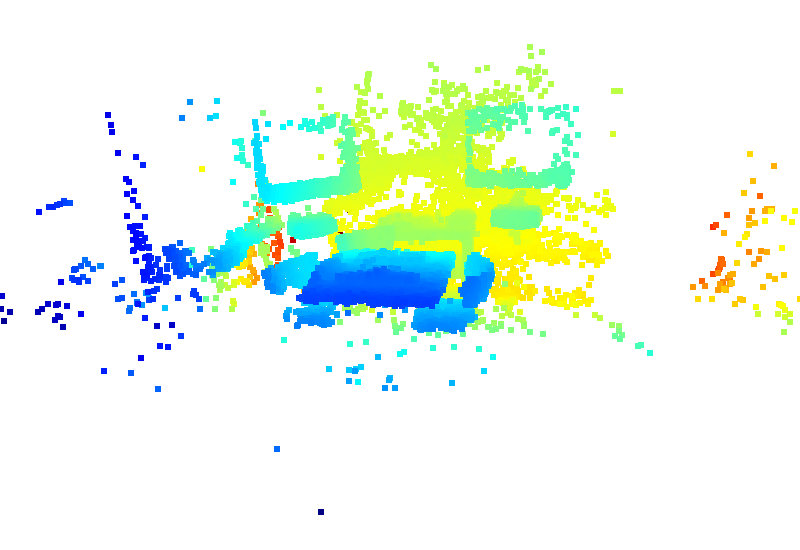
\includegraphics[width=0.2\textwidth]{images/pcs_chess.png}}\,
	\subfloat[~Fire]{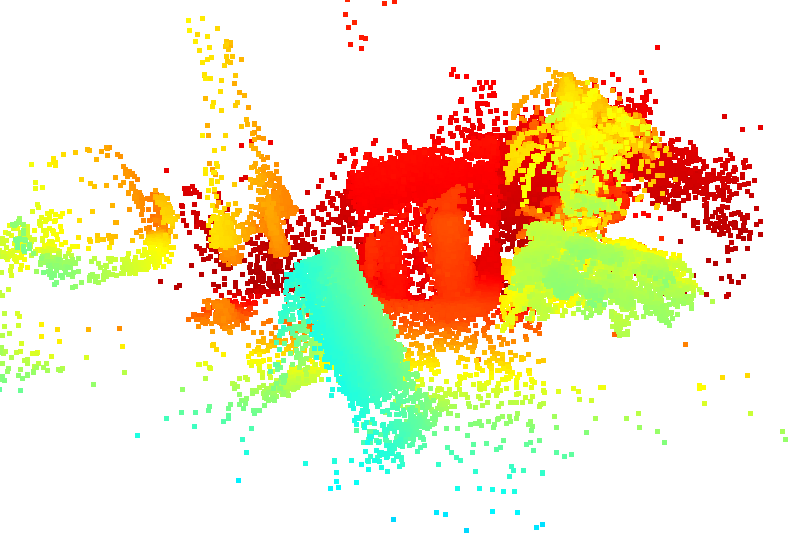
\includegraphics[width=0.2\textwidth]{images/pcd_fire.png}}\,
	\\
	\subfloat[~Pumpkin]{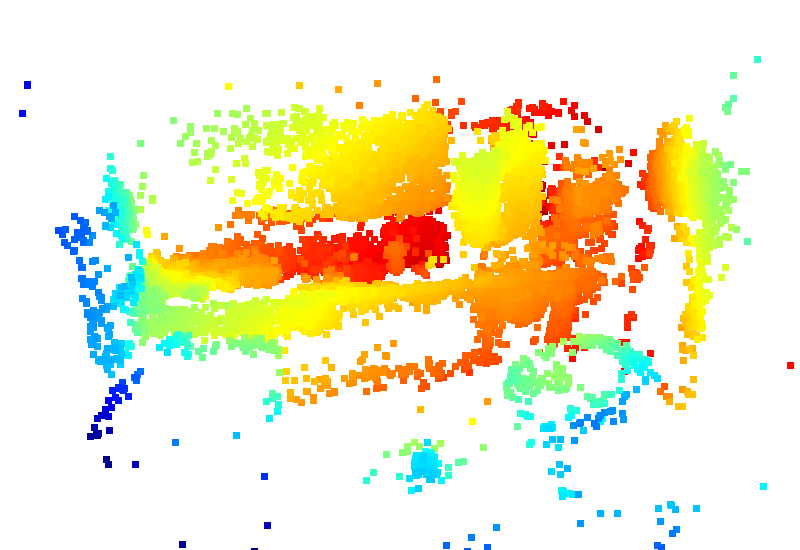
\includegraphics[width=0.2\textwidth]{images/pcd_pumpkin.png}}\,
	\subfloat[~Red Kitchen]{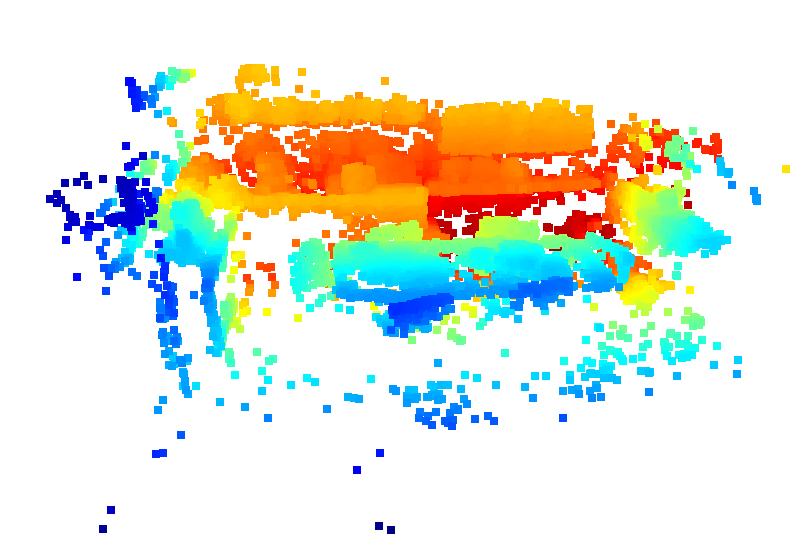
\includegraphics[width=0.2\textwidth]{images/pcd_redkitchen.png}}\,
	\subfloat[~Stairs]{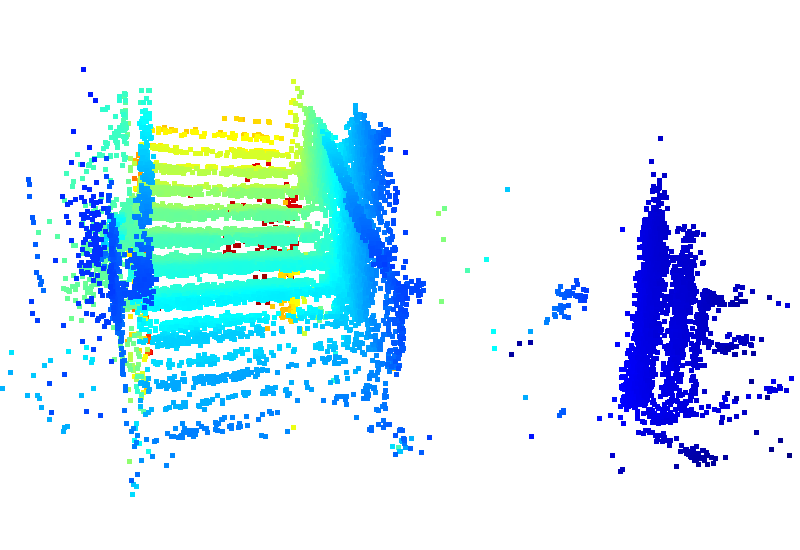
\includegraphics[width=0.2\textwidth]{images/pcs_stairs.png}}

	\end{center}
	\caption{For each scene a forest is trained with the hyperparameters stated in Table~\ref{tab:params-forest}. The forest 
	is then evaluated for $500$ test images with each having $5,000$ sample pixels. For each pixel the corresponding
	3D world coordinate is obtained. The resulting point clouds are displayed in sub-figures (a)-(e). }
	\label{fig:pointclouds}
\end{figure}

\subsection{Image to World Point correspondences} \label{subsec:eval-forest}
The forests exhibits the basic ability to predict 3D world coordinates based on 2D image pixels and 
qualitative results are shown in Figure~\ref{fig:pointclouds}. The point clouds 
allow to recognize the scenes even by a sparse number of utilized sample pixels. 

However, most scenes show areas where no 3D coordinates
were predicted. This could be attributed to a false prediction of 3D points. Due to the fact that the forest is 
trained on known world coordinates, the assignment of a pixel to a world point that is actually present in the 
scene is possible. 

\begin{table}
	\begin{center}
	\begin{tabular}{|l|c|}
	\hline
	Scene & Average Error [m]\\
	\hline\hline
	Chess 		& 	$1.079 \pm 0.388$ \\
	Fire 		& 	$0.893 \pm 0.313$	\\
	Pumpkin 	& 	$1.413 \pm 0.615$ \\
	Red Kitchen 	& 	$1.705 \pm 0.854$ \\
	Stairs 		& 	$1.496 \pm 0.753$ \\
	\hline
	\end{tabular}
	\end{center}
	\caption{Average Error and standard deviation in meters between the predicted 3D world coordinates of the 
	forest trained with 
	'Depth Adaptive RGB' features and the respective ground truths using the $\ell^2$-norm. A total of
	$500$ images each with $5,000$ sample pixels is used for evaluation for each scene.}
	\label{tab:forest-error}
\end{table}

Another explanation are invalid values during feature generation. Correspondences that could not be predicted are
caused by the fact that sample pixels are potentially shifted out of the image frame or correspond to an invalid depth value. 
Predicting the 3D world coordinates for all scenes, the forests exhibit $91.2\%$ valid predictions on average. 
This implies that a forest is capable of finding valid correspondences.

\begin{figure*}
	\begin{center}
	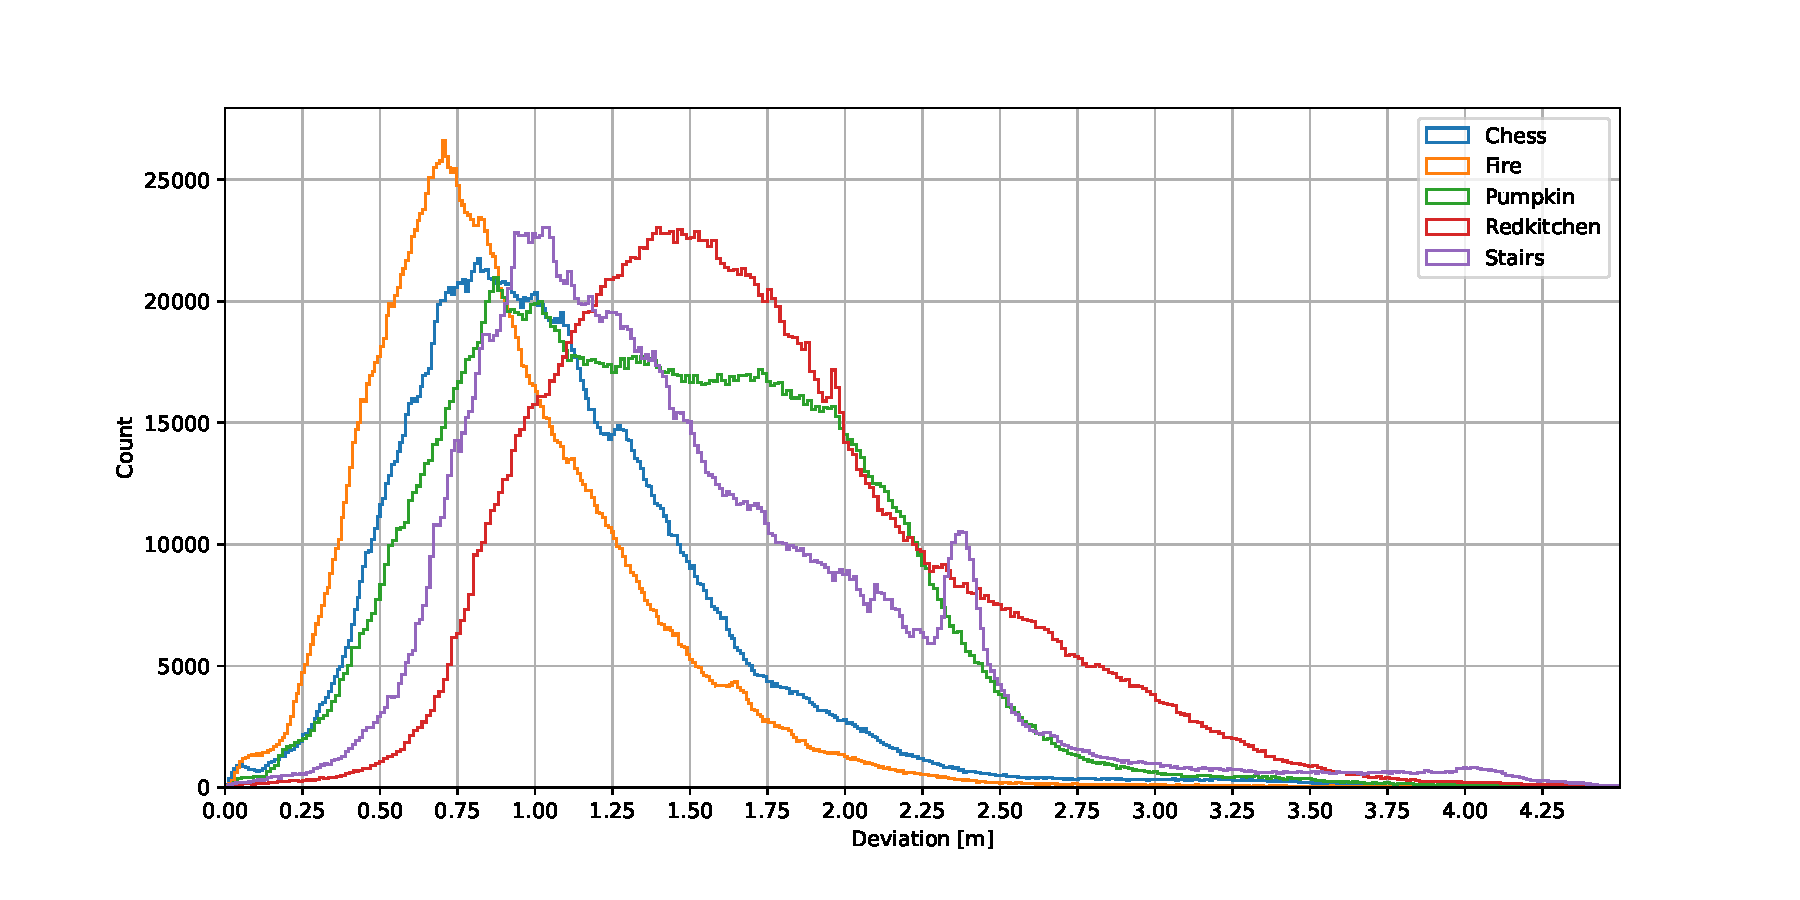
\includegraphics[width=\textwidth]{images/hist.pdf}
	\end{center}
	\caption{The histogram shows the average error of the predicted 3D world coordinates of each tree in a forest. }
	\label{fig:error-hist}
\end{figure*}

To further investigate these findings, the predicted coordinates of the forest are compared to the known ground truths using 
the $\ell^2$-norm. In Table~\ref{tab:forest-error} the error in meters and corresponding standard deviation indicates rather large 
deviations. It varies among $1.705$m for \textit{Red Kitchen} to $0.893$m for the scene \textit{Fire}. This suggests that the mapping is not as precise
as desired. By looking at the histogram of accumulative errors for each scene in Figure~\ref{fig:error-hist}, the 
previous observations are confirmed. It can therefore be expected that the majority of poses that will be predicted by the 
RANSAC algorithm deviate more than $5$cm and $5^\circ$.

Comparing the average deviations for each scene to the findings of Shotton et al.~\cite[Table 1]{shotton2013}, similarities appear.
The camera poses estimated by their implementation show the best results for the scenes "Chess" and "Fire". 
This is also indicated by the findings of the forests in this section. Since no precise measurements were
made in~\cite{shotton2013} a direct comparison of the predicted world coordinates is not possible. It is to 
be expected, that the obtained camera poses in the following section follow the same trend. 

\begin{table*}
	\begin{center}
	\begin{tabular}{|l|l|c|c|c|c|c|}
									\hline
									&               & Chess & Fire &  Pumpkin & Red Kitchen & Stairs \\ \hline\hline
	\multirow{2}{*}{Error}          & Translational [m] & $0.92 \pm 1.09$    & $0.68 \pm 0.78$     & $1.41 \pm 1.49$ & $1.89 \pm 1.31$ & $1.48 \pm 1.25$     \\ 
									& Angular [°]       & $58.52 \pm 61.85$    & $40.06 \pm 44.83$      & $66.44 \pm 65.79$      & $91.01 \pm 59.82$         & $74.59 \pm 65.92$     \\ \hline \hline
	\multirow{3}{*}{\makecell[l]{Correct \\ Poses [\%]} }  
									& $0.05m, 5^{\circ}$      &   $14.25$    &    $\boldsymbol{18.25}$  &       $10.25$         &      $4.6$      &    $7.8$    \\  
									& $0.1m, 10^{\circ}$      &    $25.75$   &  $\boldsymbol{29.75}$    &   $20.25$    &    $9.2$    &     $12.2$            \\
									& $0.15m, 15^{\circ}$      &     $33.8$  &   $\boldsymbol{38.8}$   &  $25.75$     &      $10.8$      &      $14.2$  \\
	\hline
	\end{tabular}
	\end{center}
	\caption{For each scene the camera poses are predicted and compared to the ground truth. The average translational 
	and angular	error are shown as well as the related standard deviations. The amount of correctly classified poses
	is listed in the lower part of the table for different thresholds. }
	\label{tab:pose-error}
\end{table*}

\subsection{Camera Pose Predictions}
% tranlational, angular error, vgl shotton
% best chess fire - vgl shotton bzw Baum
% warum so schlect?? szene aussehen
The predicted camera poses show rather large deviations from the ground truths as shown in Table~\ref{tab:pose-error}.
All scenes exhibit deviations with more than $0.68$m and $40.06^\circ$ which is fairly inaccurate. However, this is
to be expected regarding the results of the forests stated in Subsection~\ref{subsec:eval-forest}. Having large deviations 
of the image to world correspondences already, the prediction of related camera poses based on these values can not lead
to higher accuracies. 

Concerning the scenes \textit{Chess} and \textit{Fire}, the translational and angular error of the camera poses 
are the smallest. 
This is coherent with the precision of the predicted point correspondences of the previous subsection. 
That indicates that more precise regression forests lead to smaller error of the estimated camera pose 
by the RANSAC optimization. 

The scenes that exhibit the highest amount of correctly classified poses are \textit{Chess} and \textit{Fire}. 
The worst is provided by the scene \textit{Red Kitchen} where a lot of specularities and reflections are 
present. In the scene \textit{Stairs} many repeating patterns and ambiguities occur. This could explain the bad results 
in comparison to the other scenes.

With increasing tolerance of a pose to be classified as \textit{correct} the percentage of correct poses increases. 
Given a maximum of $5$cm and $5^\circ$ the results can not compete with~\cite{shotton2013}. Nevertheless, the trends found in 
the data sets could be reproduced. The only exception is that the \textit{Fire} scene performs better in our implementation 
which can be addressed to the performance of the respective forest shown in Subsection~\ref{subsec:eval-forest}.


\section{Conclusion}
To estimate the pose of a camera a regression forest with consecutive RANSAC optimization is utilized. Pixels are sampled from
random images of a scene and corresponding 3D world coordinates are predicted by the regression forest. Subsequently, 
the RANSAC algorithm initializes a number of camera pose hypotheses and refines them. To verify the results, the 7-scenes data 
set is used which consists of seven different 3D scenes. The predicted camera poses are then evaluated
using the translational and angular error. These findings are compared to the results of Shotton et 
al.~\cite{shotton2013}. 

The best camera pose predictions were obtained for \textit{Fire} and \textit{Chess} and the worst for \textit{Red Kitchen}
and \textit{Stairs}. Our results show the same trend as in~\cite{shotton2013}. However, our approach is not able
to achieve a similar amount of correctly classified poses. This can be addressed to the larger deviations of predicted
2D-3D correspondences by the trained forests. 

There is certainly potential to optimize our implementation in order to increase the overall accuracy of predicted camera poses.
For the future an optimization of the utilized hyperparameters could be beneficial. Additionally, other feature types may be 
of interest.

\section*{Abbreviations}
\begin{acronym}
	\acro{SIFT}{Scale-Invariant Feature Transform}
	\acro{SLAM}{Simultaneous Localization and Mapping}
	\acro{SURF}{Speeded Up Robust Features}
\end{acronym}

{\small
\bibliographystyle{ieee_fullname}
\bibliography{egbib}
}

\end{document}
